% D04-010. PDR-05 §5, открытое описание девяти органов.
\section{Аналитические органы направления мощности}
\label{sec:ch5_analytical_organs}
\conceptsource{Статья 5, раздел 5. Сохранены пять исходных
семейств и четыре дополнительных открытых алгоритма.
Это органы сравнения, а не девять заявленных новых изобретений.
Закрытый адаптивный орган описан только на уровне
раскрытых физических принципов.}

(Примечание автора: Пометка на будущее. Органы так же описаны в разделах ранее, то ли во втором, то ли ещё где-то, надо будет это потом корректно расположить, так как тут и подробнее сейчас, но тогда не станет ли он пустым ранее? Пока что прям решать не надо этот вопрос, оставим здесь описание. Но в будущем – обязательно требуется. Вроде оно не противоречит тому, но всё же, надо не забыть.)

(Примечание автора: И надо будет где-то здесь добавить пометки на то, откуда вообще это взялось? Ссылки на литературу какую-то и т.д. Вроде бы как раз исследования поисковые проводились, где-то может есть файлы в текущей базе. Ну или надо будет поискать. Сразу, если быстро найти не получится – и не надо, прост оставить задачу на это, что надо тут тоже обязательно не забыть.)



В единой методике проверки РНМ используется
сопоставление с несколькими аналитическими органами.
Они различаются поляризующими величинами,
учётом амплитуды, способом выделения вектора
и использованием предыстории.
Такие различия могут приводить
к разным ответам на одном переходном процессе.

В отличие от общего рассмотрения устройств
в главе~\ref{ch:bavr_modernization},
здесь задаются конкретные расчётные варианты,
используемые в сопоставлении.
Параметры относятся к этой конфигурации опыта
и не выдаются за неизменные уставки
всех промышленных терминалов.

\subsection{Векторная основа и выбор поляризующей величины}
\label{sec:ch5_vector_basis}
\conceptsource{Статья 5, однопериодная фильтрация и состав
входов органов. Общий расчёт симметричных составляющих
уже введён в главе 4 и не повторяется как новая разработка.}

Для полнопериодных органов используются
комплексные векторы первой гармоники,
вычисляемые по скользящему периоду измерений.
При частоте 50~Гц его длительность составляет 20~мс.
Для органов прямой последовательности
из фазных величин рассчитываются
$\dot{U}_1$ и $\dot{I}_1$
по преобразованию из
подраздела~\ref{sec:ch4_sequence_features}.

Угловая характеристика сравнивает
положение токового вектора относительно
поляризующего напряжения.
Линия максимальной чувствительности
задаёт середину рабочего сектора.
Изменение поляризующей величины
меняет и смысл отсчитываемого угла,
поэтому фазный орган с линейным напряжением
и орган прямой последовательности
рассматриваются отдельно.

Угловые характеристики показаны
на рисунке~\ref{fig:ch5_pdr_characteristics}.
Во всех полях действительная ось направлена вправо,
мнимая вверх. Поляризующий вектор каждого поля
совмещён с положительной действительной осью.
При такой общей опоре видна разница
между углом положения тока
и разностью аргументов в рабочем условии.

(Примечание автора: Вот не знаю, лучше бы всегда базисный вектор распологать вверх, чтобы «положительное» направление всегда смотрело в одну сторону. Предлагаю всё же переделать рисунки, чтобы базис «нормальный ток» всегда был в верхнем правом базисе. А уж где находится при этом напряжение или что-то другое – отдельный вопрос. Можно бы эти рисунки не трогать напрямую. Или для второго как-то два нарисовать, мол повёрнутый для «однотипности представлений» и потом все представлять вот так, чтобы прямое направление было вправо-вверх. В общем осмысли, как это правильнее изобразить и сделать. Ибо момент важный, а то развёрнутость мешает воспринимать их единым образом.)

\begin{figure}[p]
 \centering
 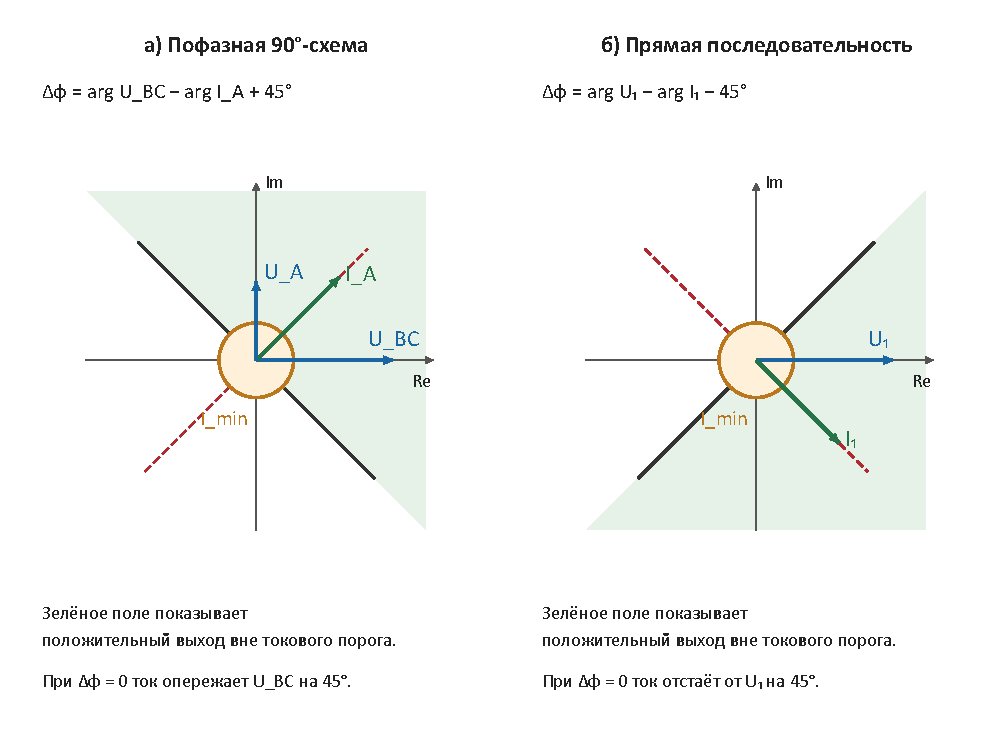
\includegraphics[width=\textwidth]{figures/ch05/ch05_angular_characteristics.pdf}
 \caption{Поясняющие схемы угловых критериев РНМ.
 Зелёная область соответствует положительному выходу,
 размеры токового порога условные.
 Напряжения на панели а показаны для симметричного режима
 с прямым чередованием фаз}
 \label{fig:ch5_pdr_characteristics}
\end{figure}
\figurereview{Поясняющий черновик D06-004 по формулам статьи 5
и раскрытой реализации угловых органов.
Вместо разнородных опор исходного рисунка 3 заданы явные Re/Im.
При UBC вдоль Re центр тока IA равен +45 градусам,
при U1 вдоль Re центр I1 равен -45 градусам.
Проверены непосредственной подстановкой в комплексные выражения.
Это схема принципа, не измеренные точки и не результат нейросети.
Исходный рисунок статьи сохранён в материалах статьи.}

\subsection{Угловые органы по фазам и прямой последовательности}
\label{sec:ch5_angular_organs}
\conceptsource{Статья 5, пофазный угловой орган и орган
прямой последовательности. Сохранены 90-градусная схема,
логическое «И» фаз и соответствующие углы чувствительности.}

В пофазной 90-градусной схеме
току A соответствует напряжение
$\dot{U}_{BC}$, току B напряжение
$\dot{U}_{CA}$, току C напряжение
$\dot{U}_{AB}$.
Для каждой пары рассчитывается
отклонение от линии максимальной
чувствительности
\begin{equation}
 \Delta\varphi_k=
 \operatorname{wrap}_{180}
 \bigl(\arg\dot{U}_{\mathrm{pol},k}
       -\arg\dot{I}_k-\varphi_{\text{мч},90}\bigr),
 \qquad \varphi_{\text{мч},90}=-45^\circ.
 \label{eq:ch5_phase_angle}
\end{equation}
Операция $\operatorname{wrap}_{180}$
приводит угол к интервалу
от $-180^\circ$ до $180^\circ$.
Фазное условие выполнено,
если $|\Delta\varphi_k|\le90^\circ$
и модуль тока не меньше
$0{,}05I_{\text{ном}}$.
Общий положительный выход требует
выполнения этих условий
во всех трёх фазах.

Такой способ объединения сохраняет
самостоятельный контроль каждой пары.
При несимметричном или однофазном
наладочном режиме условие одной
из фаз может нарушиться,
даже если другие пары находятся
в рабочем секторе.
Поэтому результат логического «И»
не совпадает автоматически
с оценкой общего вектора
прямой последовательности.

Для последней используется
\begin{equation}
 \Delta\varphi_1=
 \operatorname{wrap}_{180}
 \bigl(\arg\dot{U}_1-\arg\dot{I}_1
       -\varphi_{\text{мч},1}\bigr),
 \qquad \varphi_{\text{мч},1}=45^\circ.
 \label{eq:ch5_pos_angle}
\end{equation}
Прямой выход формируется
при $|\Delta\varphi_1|\le90^\circ$
и $|\dot{I}_1|\ge0{,}05I_{\text{ном}}$.
Здесь одно условие применяется
к согласованной величине,
полученной из всех фаз.
Обратная и нулевая последовательности
не входят в этот токовый вектор.

\subsection{Мощностные критерии}
\label{sec:ch5_power_organs}
\conceptsource{Статья 5, пофазный и прямопоследовательный
мощностные органы. Указан рабочий момент, его масштаб
и отличие от проверки одного углового сектора.}

(Примечание автора: Хмм… Интересно ,а почему тут применяется «Т»? Может так и было в литературе, мне прост странным кажется. Достаточно будет ответить на мой вопрос и всё, править сразу не нужно.)

Угловая проверка задаёт рабочую
полуплоскость вместе с токовым порогом.
В мощностном варианте учитываются
также модули напряжения и тока.
Для фазы A в принятой схеме
рабочая величина имеет вид
\begin{equation}
 T_A=\frac{|\dot{U}_{BC}|}{\sqrt3}
       |\dot{I}_A|
       \cos\bigl(\arg\dot{U}_{BC}
                 -\arg\dot{I}_A
                 -\varphi_{\text{мч},90}\bigr).
 \label{eq:ch5_phase_power}
\end{equation}
Аналогично рассчитываются
$T_B$ и $T_C$.
Коэффициент $1/\sqrt3$ согласует
масштаб линейной поляризующей величины
с принятым фазным базисом.
Он не является восстановлением
независимого фазного измерения.

В исследуемой конфигурации
положительный выход требует
превышения порога $P_{\mathrm{set}}$
каждым из трёх рабочих моментов.
Для двух базовых мощностных органов
исходная уставка равна 0,05
в физических относительных единицах.
При переходе к внутренним координатам
учитываются запас по току 20,
запас по напряжению 3,
линейный номинал напряжения при нормировке
и амплитудный масштаб комплексного вектора.
Соответствующий внутренний порог равен
$2\cdot0{,}05/(20\cdot3\sqrt3)\approx0{,}00096225$.
Именно согласованный с входом порог
сравнивается с рабочим моментом.
Положение внутри углового сектора
при малой амплитуде ещё
не обеспечивает выполнения
мощностного условия.
\figurereview{Уточнение D06-004 по сохранённым параметрам
массового и RTDS-расчётов и архивной функции пересчёта уставок.
Ранее вслед за подразделом 5.4 статьи было перенесено 0,0025,
хотя оно не задаёт согласованный масштаб этого опыта.
Параметр двух мощностных органов равен 0,05 RMS о.е.,
внутренний порог профиля dataset\_peak\_phasor равен 0,00096225.
Метрики под другую уставку не пересчитывались.
Полный тракт нормировки каждого исходного COMTRADE
этой скалярной проверкой не объявляется проверенным.}
(Примечание автора: Надо будет разобраться, пока оставляют сей вопрос за агентами.)

Для прямой последовательности
вычисляется
\begin{equation}
 T_1=\operatorname{Re}
 \left\{\dot{U}_1
       \left(\dot{I}_1e^{j\varphi_{\text{мч},1}}\right)^*
 \right\},
 \qquad m_1=T_1-P_{\mathrm{set}}.
 \label{eq:ch5_pos_power}
\end{equation}
Неотрицательный запас $m_1$
соответствует положительному
мощностному условию.
Угол, порог и масштаб входных
величин задаются согласованно.
Сам численный запас
не равен вероятности правильного
распознавания направления.

\subsection{Адаптивный орган и напряжение предыстории}
\label{sec:ch5_adaptive_organ}
\conceptsource{Статья 5. Раскрытая физическая структура
алгоритма-учителя, память напряжения и динамические пороги.
Закрытая коммерческая реализация не восстанавливается
по этим принципиальным выражениям.}

(Примечание автора: Вероятно информация будет скрыто до уровня той, что приведена в руководстве эксплуатации ООО «АПС», пока вопрос открытый и решу сам. Прост оставить напоминалку. Хотя… Вроде бы и нормально. Тогда прост стоит сказать о том, что данная методика является базисом в самых современных терминалах БАВР – поэтому обучение происходит на нём, ссылку на наше РЭ, если что приведу потом сам. Ну и какие-то слова о том, что более подробная информация об алгоритмах является конфиденциальной информацией и здесь не приводится. Но пометку всё равно оставь, вероятно потом сам перепишу описание алгоритма)

При близком повреждении текущее
поляризующее напряжение может
сильно уменьшиться.
Адаптивный орган использует
величины прямой последовательности
и информацию о предшествующем режиме.
Принцип формирования
поляризующего вектора записывается как
\begin{equation}
 \dot{U}_{1,\mathrm{pol}}
   =\dot{U}_1+k_{\mathrm{mem}}
                    \dot{U}_{1,\mathrm{hist}}.
 \label{eq:ch5_memory_voltage}
\end{equation}
В рассматриваемой постановке
глубина предыстории составляет
десять периодов.
При её отсутствии в начале
регистрации используется первая
доступная полнопериодная оценка.

Токовый порог связывается
с предшествующей нагрузкой
\begin{equation}
 I_{\mathrm{th}}=
 \max\bigl(I_{\mathrm{min}},
            k_I|\dot{I}_{1,\mathrm{hist}}|\bigr),
 \qquad I_{\mathrm{min}}=0{,}01I_{\text{ном}}.
 \label{eq:ch5_adaptive_threshold}
\end{equation}
Также изменяется рабочий угол.
Такая структура позволяет
рассматривать малые токи выбега
и потерю текущей поляризации
с учётом предшествующего режима.

Использование этого органа
как учителя задаёт начальную
автоматическую разметку.
Его ответ не принимается
за безошибочный физический эталон.
В дальнейшем он сопоставляется
с другими органами и экспертным
разбором самих осциллограмм.

Мощностной критерий и принцип памяти
показаны на рисунке~\ref{fig:ch5_power_and_memory}.
При заданном модуле поляризации
порог рабочего момента задаёт прямую границу
в плоскости токового вектора.
На второй панели показано сложение
текущего и взвешенного предшествующего напряжений.
Оно объясняет происхождение поляризующей величины,
но не задаёт полную характеристику
адаптивного органа с его динамическими порогами.

\begin{figure}[p]
\centering
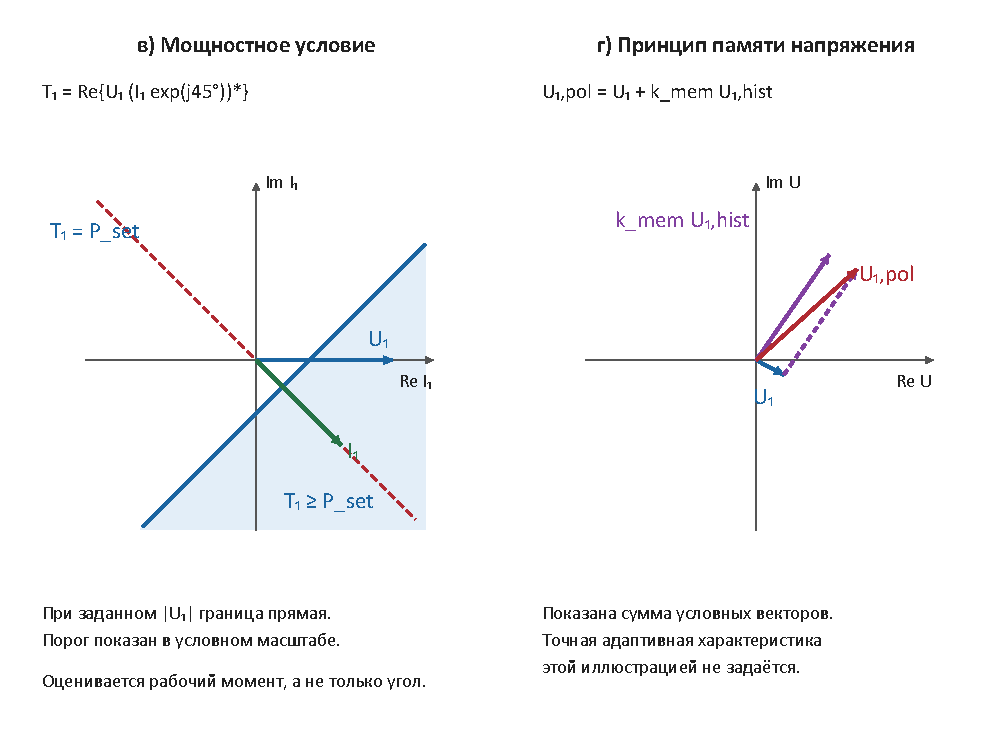
\includegraphics[width=\textwidth]{figures/ch05/ch05_power_and_memory.pdf}
\caption{Мощностное условие и принцип формирования
напряжения с памятью.
Масштаб порога и векторы условные,
токовый пуск проверяется отдельно}
\label{fig:ch5_power_and_memory}
\end{figure}
\figurereview{Поясняющий векторный черновик по раскрытым формулам,
без восстановления закрытой адаптивной характеристики.
Не подменяет испытания органов и не иллюстрирует измеренные
траектории. При необходимости автор может улучшить оформление,
сохранив указанные опоры и направления стрелок.}

\subsection{Двухвыборочная оценка вектора}
\label{sec:ch5_two_sample}
\conceptsource{Статья 5, открытый двухвыборочный алгоритм
по принципу Сивокобыленко. Сохранены формула ортогонализации
и различие времени оценки и доступности второй выборки.}

(Примечание автора: Что-то только сейчас задумался. А где-то в начале раздела сказано, что приводятся далее различные алгоритмы, которые были отобраны при анализе… Сети условно? Или чёт такое, а то перечисляются, а с какой стати мы их взяли, зачем? Это не к данному алгоритму, а скорее в целом, прост тут вопрос возник, а то он из базовых уже сильно выбивается и не совсем понятно, откуда взялся.)

Более короткий измерительный интервал
получается при оценке вектора
по двум отсчётам.
Пусть $x_0=x(t-h)$,
$x_1=x(t)$ и $\theta=2\pi fh$.
Используется выражение
\begin{equation}
 \dot{X}^{(2)}=
 x_0+j\frac{x_0\cos\theta-x_1}{\sin\theta}.
 \label{eq:ch5_two_sample}
\end{equation}
При $h$ около 1~мс
оно задаёт субцикловую оценку
для выбранной частоты.
После восстановления
недостающей фазной величины
выделяются $\dot{U}_1$
и $\dot{I}_1$.
В исследуемом варианте
применяется рабочий угол $60^\circ$
и сектор $\pm90^\circ$.

Оценка относится к первой
из двух выборок,
а вычислить её можно
после получения второй.
Эти моменты различаются на $h$.
Кроме того, формула использует
заданную частоту и короткий фрагмент,
поэтому шум, апериодическая
составляющая и отклонение частоты
могут заметно влиять на результат.
Короткий интервал не означает
одинакового качества
на всех переходных режимах.

(Примечание автора: А какой h мы тут выбрали в итоге? А то угол задан, а другое и почему именно такое?)


\subsection{Пятивыборочный орган с памятью напряжения}
\label{sec:ch5_five_sample}
\conceptsource{Статья 5, пятивыборочный орган.
Оценка производной в центре окна, восстановление вектора,
поляризация памятью и причинная доступность результата.}

В пятиточечном варианте
используются отсчёты
$x_0,\ldots,x_4$ с шагом $h$.
Оценка относится к центру
этого фрагмента.
Для синусоидальной основы
рассчитываются
\begin{equation}
 x_c=\frac{\sum_{k=0}^4x_k}
 {1+2\cos\theta+2\cos2\theta},
 \qquad
 \dot{x}_c\approx
 \frac{x_0-8x_1+8x_3-x_4}{12h},
 \label{eq:ch5_five_sample_derivative}
\end{equation}
а затем комплексная величина
\begin{equation}
 \dot{X}^{(5)}=x_c-j\frac{\dot{x}_c}{2\pi f}.
 \label{eq:ch5_five_sample_vector}
\end{equation}

По токам формируется
$\dot{I}_1^{(5)}$,
для поляризации используется
полнопериодный вектор
напряжения памяти.
Мощностное условие строится
по соответствующему рабочему моменту
с углом $60^\circ$.

При шаге около 1~мс
пять выборок охватывают около 4~мс.
В момент центра окна
последние две ещё не получены,
поэтому выдача результата
возможна не ранее чем через
два шага после этого центра.
К этому геометрическому сдвигу
дополнительно относится
готовность поляризующего канала
и остальная логика органа.

(Примечание автора: И да, что тут, что в предыдущем – точно надо писать, откуда мы всё это взяли и почему такое… То есть ссылки на литературу.)

\subsection{Дополнительная ветвь при несимметрии}
\label{sec:ch5_unbalance_branch}
\conceptsource{Статья 5, открытая реализация по принципу
БМРЗ-БАВР. Различаются основное мощностное условие
и целенаправленная корректирующая ветвь.}

В комбинированном варианте
по принципу БМРЗ-БАВР
основное условие определяется
активной мощностью
прямой последовательности
\begin{equation}
 P_1=\operatorname{Re}
             \{\dot{U}_1\dot{I}_1^*\}.
 \label{eq:ch5_unbalance_power}
\end{equation}
При повышенной обратной
последовательности напряжения
добавляется проверка величины
\begin{equation}
 I_{p,1}=|\dot{I}_1|
 \sin\bigl(\arg\dot{U}_1-\arg\dot{I}_1\bigr).
 \label{eq:ch5_unbalance_current}
\end{equation}
В рассматриваемой конфигурации
ветвь используется при
$|\dot{U}_2|>0{,}08U_{\text{ном}}$.
Превышение
$I_{p,1}>0{,}05I_{\text{ном}}$
относится к обратному состоянию.
В остальных режимах
применяется основной критерий
с порогом 0,001
и угловым гистерезисом $8^\circ$.

Дополнительная проверка
меняет ответ в определённой
физической области.
Она не рассматривается
как независимый голос,
который можно произвольно
прибавить к остальным органам.
Это открытая исследовательская
реализация принципа,
а не полное описание
любого серийного устройства.

(Примечание автора: Думаю, что тут, что в других надо бы везде картинки принципа работы органов, тут можно векторку построить, а двухвыборочном и пятивыборочном… Пока не знаю, но наверное что-то тоже. В общем, какие-то поясняющие картинки. Но уж тут точно что-то да можно бы.)


% D06-005 R5-03 BEGIN
\ifdefined\AuthorReview
\par\smallskip\begingroup\small\raggedright\color{red!60!black}
\noindent\textbf{Примечание рецензента [R5-03], ясность условий сравнения.} После исправления основной мощностной уставки остаётся неоднозначным масштаб порога 0,001 у БМРЗ-варианта выше. Кратко указать физическую величину и базис этого порога. Для девяти органов полезна компактная сводка фактически использованных уставок и памяти, с отсылкой к подробным формулам. Сравнение относится к этим настройкам; из него не следует, что каждый принцип испытан при оптимальных уставках. Новую настройку или пересчёт сейчас не выполнять.\par\endgroup\smallskip
\fi
% D06-005 R5-03 END
(Примечание автора: Пока агентам самим разобраться.)

\subsection{Адаптация принципа БАВР-072}
\label{sec:ch5_bavr072_proxy}
\conceptsource{Статья 5. Открытый memory proxy при отсутствии
синхронного измерения резервного источника в архивах.
Результат не называется точной копией серийного БАВР-072.}

При использовании информации
о резервном источнике
состав доступных измерений
отличается от рассмотренных
архивных записей.
В них такой синхронный канал
отсутствует.
Для воспроизводимого сопоставления
используется открытая адаптация
с поляризующей величиной
\begin{equation}
 \dot{U}_{\mathrm{pol}}=
 \dot{U}_1+0{,}3\dot{U}_{1,\mathrm{mem}}.
 \label{eq:ch5_bavr072_proxy}
\end{equation}
Напряжение памяти имеет
глубину десять периодов.
Рабочий момент рассчитывается
по этому поляризующему вектору
и току прямой последовательности
с рабочим углом $45^\circ$.

Такой вариант позволяет
рассмотреть влияние памяти
при снижении текущего напряжения.
Он не восстанавливает
отсутствующее измерение
резервного источника
и не является точной
копией серийного терминала.
Именно в таком ограниченном
смысле он используется
как один из органов сравнения.

(Примечание автора: Ну и надо бы тогда сказать, что остальное аналогично какой-то базе (ссылка на что-то выше)?.)